\documentclass{article}

% Language setting
% Replace `english' with e.g. `spanish' to change the document language
\usepackage[english]{babel}
\usepackage{wrapfig}
% Set page size and margins
% Replace `letterpaper' with`a4paper' for UK/EU standard size
\usepackage[letterpaper,top=2cm,bottom=2cm,left=3cm,right=3cm,marginparwidth=1.75cm]{geometry}

% Useful packages
\usepackage{amsmath}
\usepackage{graphicx}
\usepackage[colorlinks=true, allcolors=blue]{hyperref}

\title{Hotel Reviews Sentiment Analysis}
\author{Chongyi Zheng, Zeyu Zhang, Suning Chen, Peifeng He}

\begin{document}
\maketitle

\section{Introduction}

Users write a lot of reviews for the hotels they have stayed in and rate these hotels. Our interest is to determine the user's attitudes towards this hotel only based on the sentiment in their reviews. To achieve this goal, we analyzed about 20,000 user review data with a text length of 13543965 (after cleaning). In order to compare the accuracy between different models and pick the most suitable mode, we utilized several different models to train our data, including Naive Bayes, K-Nearest Neighbors, Decision Tree, Random Forest, and Bidirectional LSTM. We predicted the attitudes of the users corresponding to different reviews by using these models. The results are classified as satisfied (labeled as Good), unsatisfied (labeled as Bad), and neutral. Among them, Bidirectional LSTM predicts more accurate results, not only can analyze the positive and negative attitudes of users but also can detect whether users are neutral or not. The code used in this article is at: https://github.com/harryzcy/COMP562-project.

\subsection{Motivation}
The reason we chose this topic is that sentiment analysis has a wide range of uses in society and is also very important. In the absence of a numerical score, we are able to obtain the attitude of the author in a sentence. This allows us to test whether the score given by the user corresponds to his rating. Moreover, our model is not limited to judging hotel reviews but can be extended to other areas, such as inferring a person's mood during AI-human interaction.

\subsection{Related Work}
The field of sentiment analysis has been extensively researched in the past few decades. Many different techniques have been proposed for this task, including both traditional machine learning approaches and more recent deep learning methods. One of the most common techniques for sentiment analysis is the use of a Bidirectional Long Short-Term Memory (BiLSTM) network. BiLSTM networks are a type of recurrent neural network (RNN) that are able to effectively capture contextual information from both past and future words in a sentence. This makes them well-suited for the task of sentiment analysis, where the meaning of a word may depend on its context within the sentence.
Other machine learning techniques applied to sentiment analysis include naive Bayes and random forests. Naive Bayes is a simple probabilistic classifier that makes use of Bayes' theorem to predict the sentiment of a given sentence. It has the advantage of being relatively easy to implement and interpret, but can sometimes struggle with the more complex or nuanced sentiments. Random forest, on the other hand, is a classification algorithm consisting of many decision trees. They are able to capture complex non-linear relationships in the data and have been shown to perform well on many natural language processing tasks, including sentiment analysis. However, they can be computationally expensive to train and may not be suitable for real-time applications.

\section{Hotel Review Sentiment Analysis}

\subsection{Data Visualization}

\begin{figure}[h]
\centering
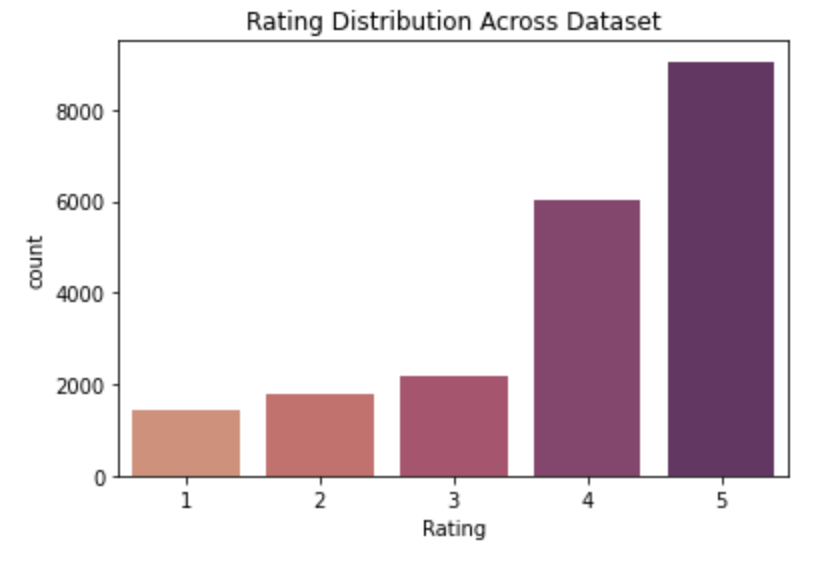
\includegraphics[width=0.6\linewidth]{distribution.png} 
\caption{Rating Distribution}
\label{fig:wrapfig}
\end{figure}

Our first step is data visualization. Our data set was downloaded from Kaggle. The data set contains 20492 hotel reviews and corresponding scores given by clients. We did a statistic on the ratings of the hotel, and we classified the reviews based on the rating given by those customers. Among the ratings, over 8000 clients gave a 5 (indicates that this client is satisfied) to the hotel, but there are also thousands of 1, 2, 3, and 4 in the data set.


\subsection{Data Cleaning and Text Processing}
\begin{flushleft}
We transferred ratings 4 and 5 to "Good", 3 to "Neutral", and 1 and 2 to "Bad". After we processed the sentiment analysis, this can help us to check our prediction. 

\begin{table}[h]
\centering
\begin{tabular}{m|m}
Ratings & Classification \\\hline
5 & Good \\
4 & Good \\
3 & Neutral \\
2 & Bad \\
1 & Bad
\end{tabular}
\caption{\label{tab:widgets}Rating Classification}
\end{table}
\end{flushleft}

\noindent
We also need to clean the review message. The first step is to remove uppercase letters and punctuation, which is not important in our sentiment analysis. The second step is to remove stop words in English. Those words will not indicate any preference from the user. The last step is to lemmatize the word, so different inflected of the words can be analyzed as the same word. \newline

\begin{figure}[h]
    \centering
    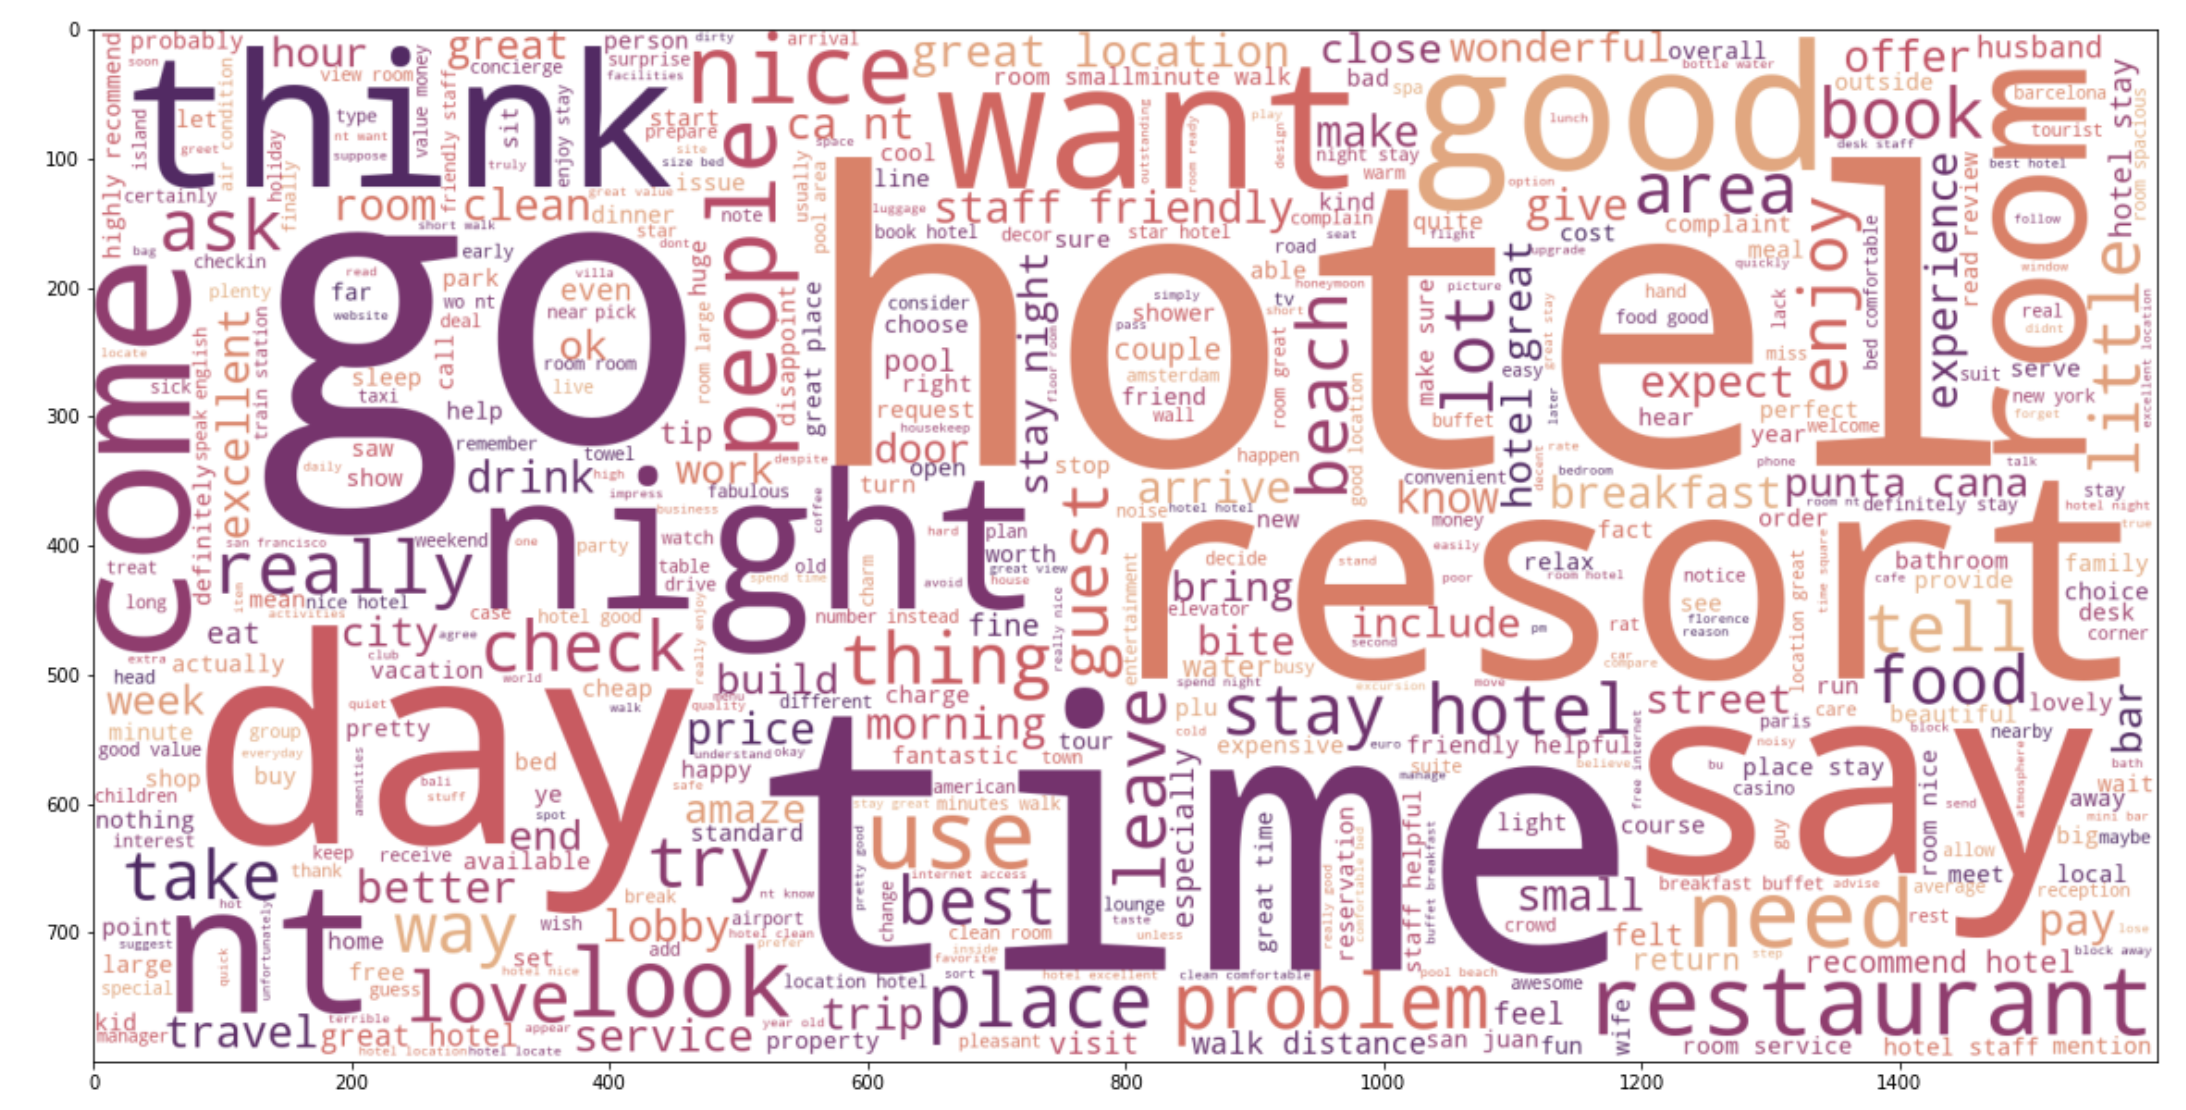
\includegraphics[width=0.6\textwidth]{wordFreqency.png}
    \caption{Word Frequency in Reviews}
    \label{fig:my_label}
\end{figure}

\noindent
The text length before cleaning is 14853861. After we cleaned the data, the text length is 13543965.

\subsection{Train and Test Data sets}

Now, review data are fully processed and ready to be trained by using the model we prepared. For each model, we use two different vectorization methods. First is "Count Vectorization", which is counting the number of occurrences of each word that appears in the data set. The second method is Tfi-df Vectorization, which not only focuses on the frequency of the words but also provides the importance of the words. \newline

\noindent
After training the data set with Naive Bayes, K-Nearest Neighbors, Decision Tree, Random Forest, and Bidirectional LSTM, we used the test data to test the results and calculate the accuracy. \newline

\noindent
Among all the models, the accuracy is around 0.8. The result from Bidirectional LSTM has a relatively higher accuracy of 0.9548. The details of the calculation are available in our code file.
\begin{table}[h]
\centering
\begin{tabular}{m|m|m}
Model name & Vectorization Method & Accuracy \\\hline
Naive Bayes & Count Vectorization & 0.8175 \\
Naive Bayes & Tfi-df Vectorization & 0.8192 \\
K-Nearest Neighbors & Count Vectorization & 0.7497 \\
K-Nearest Neighbors & Tfi-df Vectorization & 0.7741 \\
Decision Tree & Count Vectorization & 0.7370 \\
Decision Tree & Tfi-df Vectorization & 0.7287 \\ 
Random Forest & Count Vectorization & 0.8173 \\
Random Forest & Tfi-df Vectorization & 0.8141 \\
Bidirectional LSTM & / & 0.9548
\end{tabular}
\caption{\label{tab:widgets}Model Accuracy}
\end{table}

\subsection{Prediction and Application}
We also want to test these trained models on actual reviews other than the test data set. Here, we wrote three reviews by ourselves and check whether the model will make a correct prediction. \newline

\noindent
The first text message is "Excellent way stayed inn market memorial day weekend. The room is large and has great view. Great hotel great hotel, good sized". This is definitely a positive review and we labeled it as "Good". When we use our models to process this review, all of the models believe that it is "Good", which means they all make the correct prediction. \newline

\noindent
The second message is "Disgusting room with bad smell", which is obviously a negative review, so we labeled it as "Bad". When we applied our models, all the models made the correct prediction except the K-Nearest Neighbors model with the Tfi-df vectorizer, which predicts that this is a good review. \newline

\noindent
The third message is "Hard to get there, and the room is small", which is obviously a negative review, and we labeled it as "Bad" manually. When we applied our models, only three models made the correct prediction. Interestingly, the model (K-Nearest Neighbors model with the Tfi-df vectorizer) which made the wrong prediction for the previous review actually made a correct prediction this time. The other two models that made a correction prediction are the Decision Tree with Tfi-df vectorizer and Bidirectional LSTM. This is another fact that persuades us that Bidirectional LSTM is a suitable model for this data set. As a result, although we can classify this review easily, our models do not make an accurate prediction on this review. \newline

\noindent
The last message says that "Hard to get here but the scenery is wonderful", which we think is neutral. We labeled it as "Neutral" and then apply our models. This time, only one model, Bidirectional LSTM, made the correct prediction. All other models believe that this is a good review. \newline

\noindent
We now gain the result of the four predictions. We believe the most suitable model for this hotel review data set is Bidirectional LSTM. This model has the highest accuracy. Besides, it can make correct predictions on reviews relatively close to neutral (EX: the third test), and it is the only model that made correct predictions on neutral reviews.

\subsection{Conclusion and Future Study}
Bidirectional LSTM provided the highest accuracy, and this model is more sensitive than other models when the review's attitude is vague. By doing this analysis, we can use our algorithm to make a decision on the attitude of the review. \newline

\noindent
Our future research goal is to improve our model on vague reviews. When the review does not have a clear attitude or the review is "Neutral", we hope our model can still determine the attitude and provide a correct result. Following this goal, our model can then have more categories. Noted that usually there are five ratings(1, 2, 3, 4, and 5), which we can improve our model to correspond each rating into a specific class.  

\newpage
\section{References}
Yulita, I. N., Fanany, M. I., & Arymuthy, A. M. (2017). Bi-directional long short-term memory using quantized data of deep belief networks for Sleep Stage Classification. Procedia Computer Science, 116, 530–538. https://doi.org/10.1016/j.procs.2017.10.042 \newline

\noindent
Spencer, E. L. (2022, September 9). Sentiment Analysis for Brand Building: A comprehensive guide. Blog. Retrieved December 9, 2022, from https://www.revuze.it/blog/sentiment-analysis/ \newline

\noindent
Breiman, L. Random Forests. Machine Learning 45, 5–32 (2001).
https://doi.org/10.1023/A:1010933404324

\subsection{Data Set}
https://www.kaggle.com/datasets/andrewmvd/trip-advisor-hotel-reviews
\end{document}